\documentclass[a4paper,11pt]{article}

\usepackage{amsmath}
\usepackage{amssymb}
\usepackage{listings}
\usepackage{color} %red, green, blue, yellow, cyan, magenta, black, white
\definecolor{mygreen}{RGB}{28,172,0} % color values Red, Green, Blue
\definecolor{mylilas}{RGB}{170,55,241}
%\usepackage{amsthm}
\usepackage{graphicx}
\usepackage{epstopdf}
\epstopdfsetup{update}
%\usepackage{caption}
%\usepackage{subcaption}

\newcommand{\ba}{\begin{array}}
\newcommand{\ea}{\end{array}}

\newcommand{\bea}{\begin{eqnarray}}
\newcommand{\eea}{\end{eqnarray}}

\newcommand{\bc}{\begin{center}}
\newcommand{\ec}{\end{center}}

\newcommand{\ds}{\displaystyle}

\newcommand{\bt}{\begin{tabular}}
\newcommand{\et}{\end{tabular}}

\newcommand{\bi}{\begin{itemize}}
\newcommand{\ei}{\end{itemize}}

\newcommand{\bd}{\begin{description}}
\newcommand{\ed}{\end{description}}

\newcommand{\bp}{\begin{pmatrix}}
\newcommand{\ep}{\end{pmatrix}}

\newcommand{\pd}{\partial}
\newcommand{\sech}{\mbox{sech}}

\newcommand{\cf}{{\it cf.}~}

\newcommand{\ltwo}{L_{2}(\mathbb{R}^{2})}
\newcommand{\smooth}{C^{\infty}_{0}(\mathbb{R}^{2})}

\newcommand{\br}{{\bf r}}
\newcommand{\bk}{{\bf k}}
\newcommand{\bv}{{\bf v}}

\newcommand{\gnorm}[1]{\left|\left| #1\right|\right|}
\newcommand{\ipro}[2]{\left<#1,#2 \right>}


\author{Matteo Polimeno}
\date{November $28^{th}$, 2018}
\title{MATH693a\\
	Dr. Peter Blomgren\\
	HW05\\
	BFGS}
\begin{document}
\lstset{language=Matlab,%
		%basicstyle=\color{red},
		breaklines=true,%
		morekeywords={matlab2tikz},
		keywordstyle=\color{blue},%
		morekeywords=[2]{1}, keywordstyle=[2]{\color{black}},
		identifierstyle=\color{black},%
		stringstyle=\color{mylilas},
		commentstyle=\color{mygreen},%
		showstringspaces=false,%without this there will be a symbol in the places where there is a space
		numbers=left,%
		numberstyle={\tiny \color{black}},% size of the numbers
		numbersep=9pt, % this defines how far the numbers are from the text
		emph=[1]{for,end,break},emphstyle=[1]\color{red}, %some words to emphasise
		%emph=[2]{word1,word2}, emphstyle=[2]{style},    
}
\maketitle
\section*{BFGS Algorithm - Implementation and Results}

In this HW assignment we grab the file $rosenbrock2Nd.m$ from the slides and use it to implement the BFGS algorithm to find the minimum of the function.  We compare iteration count and elapsed time of the algorithm to the newton method.

\begin{center}
	\begin{tabular}{||c |c | c ||} 
		Method & Iterations & Elapsed Time (sec)\\
		\hline\hline
		Newton & 27 & 0.0608\\
		\hline
		BFGS & 131 & 0.00121\\
		\hline\hline
	\end{tabular}
\end{center}

As we see from the above table, the BFGS algorithm is faster overall in term of elapsed time, but takes more than $100$ more iterations compared to the Newton Method.
For completeness in our results, we plot the Residual 2-norm for the BFGS and we check the convergence criteria for the algorithm.

\begin{figure}[!ht]
	\centering
	\begin{tabular}{cc}
		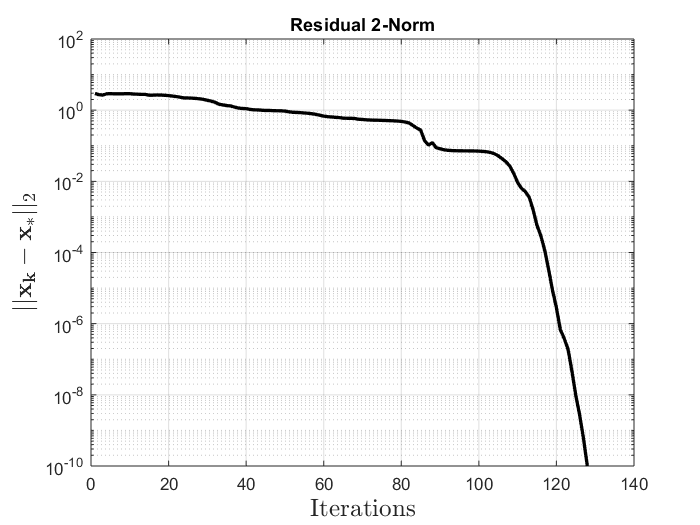
\includegraphics[width=.55\textwidth]{Residual} &\hspace{-25pt}
		(a)\\
		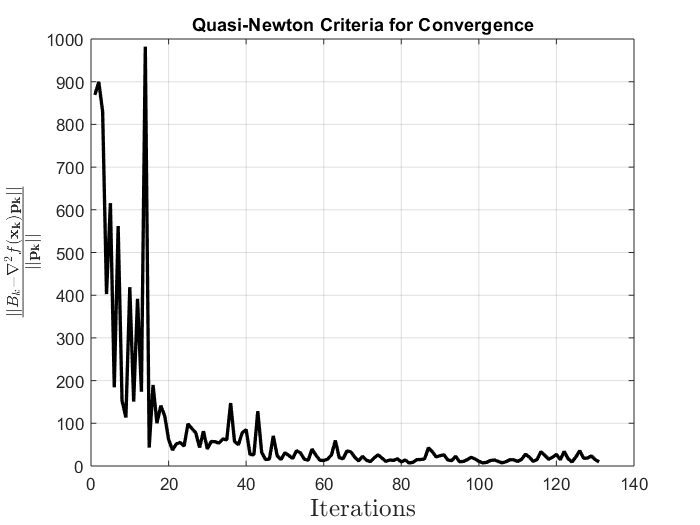
\includegraphics[width=.55\textwidth]{QN} &\hspace{-25pt} 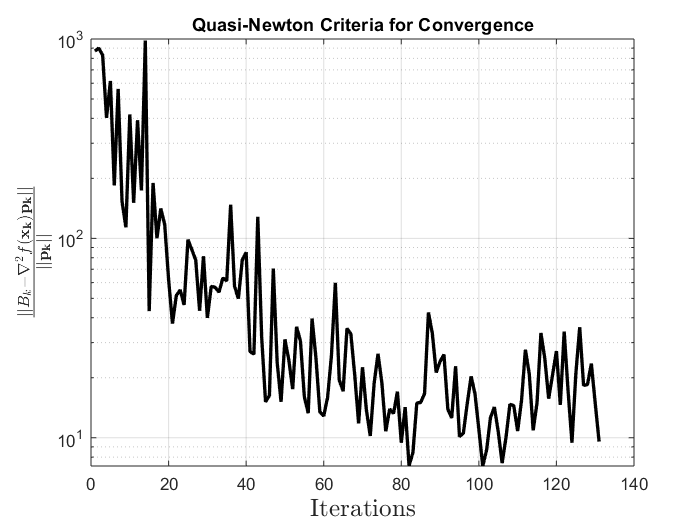
\includegraphics[width=.55\textwidth]{QN_semilogy} \\
		b) & c)\\
	\end{tabular}
	\caption{Euclidean Norm for the Residual a) and the Quasi-Newton Criteria for convergence on a linear scale b) and on a logarithmic scale c)}
	\label{}
\end{figure}

\clearpage
\section*{Appendix - Matlab Code}
\subsection*{Provided Code}
\lstinputlisting{rosenbrock_2Nd.m}
\clearpage
\subsection*{BFGS Algorithm}
\lstinputlisting{BFGS.m}
\clearpage
\subsubsection*{Linesearch}
\lstinputlisting{wolfe_strong2.m}
\clearpage
\lstinputlisting{interp2.m}
\lstinputlisting{zoom2.m}
\clearpage
\lstinputlisting{phi_prime.m}
\end{document}